% Editable source for profile.pdf, written by make_setup_profile.py from inputs/setup_profile_archived.json
\documentclass[tikz,border=6pt]{standalone}
\usepackage[T1]{fontenc}
\begin{document}
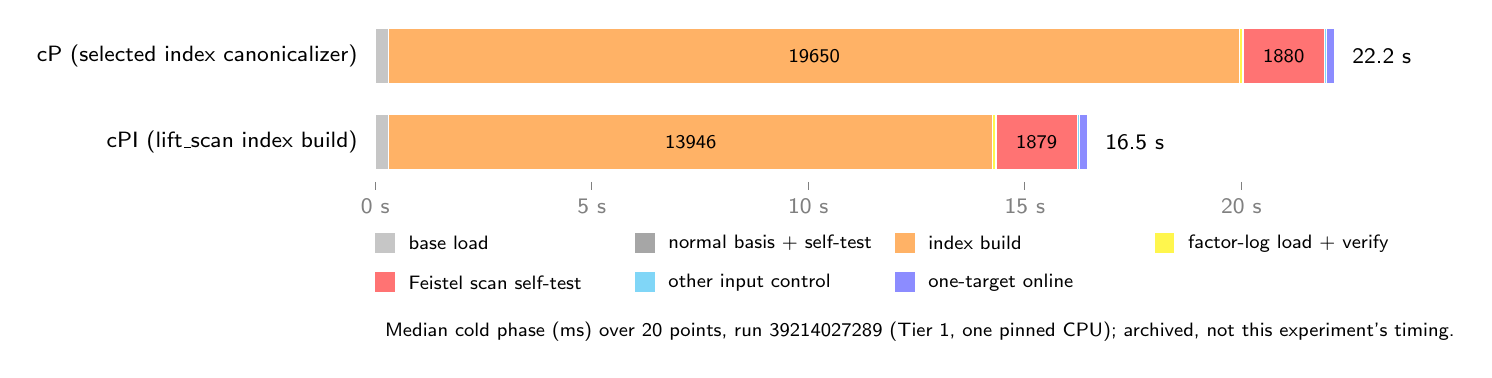
\begin{tikzpicture}[font=\sffamily\footnotesize]
\node[anchor=east] at (-0.1,0.00) {cP (selected index canonicalizer)};
\fill[gray!45,draw=white] (0.0000,-0.35) rectangle (0.1678,0.35);
\fill[gray!70,draw=white] (0.1678,-0.35) rectangle (0.1723,0.35);
\fill[orange!60,draw=white] (0.1723,-0.35) rectangle (10.9797,0.35);
\node[font=\sffamily\scriptsize] at (5.5760,0.00) {19650};
\fill[yellow!70,draw=white] (10.9797,-0.35) rectangle (11.0207,0.35);
\fill[red!55,draw=white] (11.0207,-0.35) rectangle (12.0545,0.35);
\node[font=\sffamily\scriptsize] at (11.5376,0.00) {1880};
\fill[cyan!50,draw=white] (12.0545,-0.35) rectangle (12.0864,0.35);
\fill[blue!45,draw=white] (12.0864,-0.35) rectangle (12.1865,0.35);
\node[anchor=west] at (12.2865,0.00) {22.2 s};
\node[anchor=east] at (-0.1,-1.10) {cPI (lift\_scan index build)};
\fill[gray!45,draw=white] (0.0000,-1.45) rectangle (0.1678,-0.75);
\fill[gray!70,draw=white] (0.1678,-1.45) rectangle (0.1723,-0.75);
\fill[orange!60,draw=white] (0.1723,-1.45) rectangle (7.8425,-0.75);
\node[font=\sffamily\scriptsize] at (4.0074,-1.10) {13946};
\fill[yellow!70,draw=white] (7.8425,-1.45) rectangle (7.8834,-0.75);
\fill[red!55,draw=white] (7.8834,-1.45) rectangle (8.9171,-0.75);
\node[font=\sffamily\scriptsize] at (8.4003,-1.10) {1879};
\fill[cyan!50,draw=white] (8.9171,-1.45) rectangle (8.9489,-0.75);
\fill[blue!45,draw=white] (8.9489,-1.45) rectangle (9.0487,-0.75);
\node[anchor=west] at (9.1487,-1.10) {16.5 s};
\draw[gray] (0.0000,-1.6) -- (0.0000,-1.7) node[below] {0 s};
\draw[gray] (2.7500,-1.6) -- (2.7500,-1.7) node[below] {5 s};
\draw[gray] (5.5000,-1.6) -- (5.5000,-1.7) node[below] {10 s};
\draw[gray] (8.2500,-1.6) -- (8.2500,-1.7) node[below] {15 s};
\draw[gray] (11.0000,-1.6) -- (11.0000,-1.7) node[below] {20 s};
\fill[gray!45] (0.00,-2.5) rectangle ++(0.25,0.25); \node[anchor=west,font=\sffamily\scriptsize] at (0.30,-2.38) {base load};
\fill[gray!70] (3.30,-2.5) rectangle ++(0.25,0.25); \node[anchor=west,font=\sffamily\scriptsize] at (3.60,-2.38) {normal basis + self-test};
\fill[orange!60] (6.60,-2.5) rectangle ++(0.25,0.25); \node[anchor=west,font=\sffamily\scriptsize] at (6.90,-2.38) {index build};
\fill[yellow!70] (9.90,-2.5) rectangle ++(0.25,0.25); \node[anchor=west,font=\sffamily\scriptsize] at (10.20,-2.38) {factor-log load + verify};
\fill[red!55] (0.00,-3.0) rectangle ++(0.25,0.25); \node[anchor=west,font=\sffamily\scriptsize] at (0.30,-2.88) {Feistel scan self-test};
\fill[cyan!50] (3.30,-3.0) rectangle ++(0.25,0.25); \node[anchor=west,font=\sffamily\scriptsize] at (3.60,-2.88) {other input control};
\fill[blue!45] (6.60,-3.0) rectangle ++(0.25,0.25); \node[anchor=west,font=\sffamily\scriptsize] at (6.90,-2.88) {one-target online};
\node[anchor=west,font=\sffamily\scriptsize] at (0,-3.5) {Median cold phase (ms) over 20 points, run 39214027289 (Tier 1, one pinned CPU); archived, not this experiment's timing.};
\end{tikzpicture}
\end{document}
